% Format verslag in LaTeX maken.
% Lars Aalsma, Tutor Natuur- en Sterrenkunde 2014-2015
% & Ramon Creyghton, tutor Natuur- en Sterrenkunde 2014-2016.
% & David Fokkema, staflid natuurkundepracticum, september 2017.
%
% Dit document mag naar eigen inzicht aangepast en verspreid worden.
% Her en der in dit document staan opmaak-opties en packages opgenomen, die afhankelijk van je voorkeuren kunnen worden aan- of uitgezet. Het is aan te raden je te verdiepen in de werking van deze opties (ze googlen is een start) voor je ze gebruikt.

\documentclass[11pt,a4paper]{article}

\usepackage{fouriernc}        % Dit package kiest het lettertype. Laat dit weg voor standaard Computer Modern.
\usepackage[utf8]{inputenc}   % Je kunt gewóón accenten typen, als je wilt
\usepackage[T1]{fontenc}      % Nodig om de accenten ook ín de pdf te krijgen
\usepackage[dutch]{babel}     % Figuur i.p.v. Figure, en NL afbrekingen
\usepackage{graphicx}         % Voor \includegraphics om figuren in te voegen
\usepackage{amssymb}          % Voor extra symbolen
\usepackage{amsmath}          % Voor extra ondersteuning bij vergelijkingen (zie documentatie)
\usepackage{natbib}           % Voor auteur-jaar citatie.
\usepackage{a4wide}           % Past marges aan voor A4.
\usepackage[small]{caption}   % Voor bijschriften met een iets kleinere lettergrootte dan de hoofdtekst.
\usepackage{url}              % Voor het beter weergeven van url's (lang, of met speciale tekens)
\usepackage{booktabs}         % Voor professionele tabellen
\usepackage[output-decimal-marker={,},list-final-separator={ en }]{siunitx}          % Voor het typesetten en uitlijnen van getallen en eenheden, zie documentatie
\usepackage[pdfusetitle]{hyperref}  % Voor handige links in je PDF. B.v. urls, referenties, etc.
\usepackage{physics}

\linespread{1.3}              % Iets grotere regelafstand: fijn voor degene die het nakijkt.

% \renewcommand{\arraystretch}{1.5}   % Om rijen in tabellen wat ruimer rond de tekst te maken.

%% DOCUMENT PROPERTIES
\author{Frenk Klein Schiphorst} % vul in
\title{Werkplan On-site Experiment} % Vul in.
\date{\today}

\begin{document}

\suppressfloats[t]      % Nu volgt eigenlijk de eerste pagina van het document. Je wilt dan niet beginnen met een figuur. Dit commando (suppress floats at top of the page) onderdrukt een eventueel figuur en schuift dat naar een andere positie. Dit commando geldt alleen voor de *huidige* pagina.

%%BEGIN VAN DE INHOUD VAN HET DOCUMENT

\section{Onderzoeksvraag}
Is de stopping power voor en de dracht van alfadeeltjes in lucht en helium binnen 20\% van de theoretische waarde te bepalen?

\section{Context}
Alfadeeltjes zijn hoogenergetische deeltjes die vrijkomen bij bepaalde soorten radioactief verval. Door deze hoge energie zijn ze potentieel schadelijk voor de gezondheid. De relatief hoge massa van alfadeeltjes in combinatie met de hoge energie zorgt echter ook voor een hoog ioniserend vermogen. Hierdoor zullen ze botsen met vrijwel elk deeltje dat ze tegenkomen en zijn ze veel makkelijker af te stoppen dan bijvoorbeeld gammastraling.

\section{Theorie}
Bij alfa-verval stoot een radioactieve kern een heliumkern uit. Deze heliumkernen worden alfadeeltjes genoemd. Alfadeeltjes zijn relatief veel groter en zwaarder dan bèta- en gammadeeltjes, en hebben ook een veel hogere energie. De energie wordt afgestaan door botsingen met atomen, die daardoor geëxciteerd of geïoniseerd kunnen worden. Door de hoge energie kunnen ze veel meer atomen exciteren en ioniseren dan bijvoorbeeld gammadeeltjes, omdat ze per interactie niet meteen al hun energie verliezen. De grootte en massa en de hoge energie van de alfadeeltjes zorgen echter ook voor een hoog ioniserend vermogen. Dit betekent dat ze botsen met vrijwel elk deeltje dat ze tegenkomen. Hierdoor verliezen ze hun energie veel sneller dan gammadeeltjes en kunnen ze veel minder ver doordringen in een materiaal.\par
Alfadeeltjes kunnen al gestopt worden door een velletje papier. De kans dat ze door de huid heen komen is dus ook niet zo groot. Alfastraling is daarom vooral schadelijk als de bron het lichaam binnendringt, bijvoorbeeld door inslikken.\par
Bij dit experiment wordt gebruik gemaakt van een americium-241 bron. Dit is een alfastraler. De vrijgekomen alfadeeltjes hebben een energie rond 5,5 MeV \cite{Americium241}. De precieze energieën en de percentages waarin ze voorkomen staan in tabel \ref{tab:table_1}. \par
De stopping power voor een alfadeeltje in een bepaalde stof is gedefinieerd als:
\begin{equation}
\mathrm{stopping \ power} \equiv -\frac{\mathrm{d}T}{\mathrm{d}x}
\label{eq:stopping_power}
\end{equation}
waarbij $\mathrm{d}T$ het energieverlies is en $\mathrm{d}x$ de afgelegde afstand in het materiaal. Voor de theoretische waarden voor de stopping power, zie tabel \ref{tab:table_2}.\par
Uit de energie van het uitgestoten alfadeeltje en de stopping power kan de dracht van het alfadeeltje berekend worden. De dracht geeft aan hoe ver het deeltje in een materiaal kan doordringen voordat het helemaal afgestopt is. Bij alfadeeltjes is deze dracht vrij laag, een paar centimeter. In lucht geldt de volgende relatie tussen de dracht en de energie van een alfadeeltje \cite{RangeAir}:
\begin{equation}
R_\alpha = 0,318 E_\alpha ^{3/2}
\label{eq:Range_air}
\end{equation}
Hieruit volgt voor de dracht van de meest voorkomende alfadeeltjes uit americium-241 $R_\alpha = 4.09 $ cm. Voor de dracht van dezelfde alfadeeltjes in helium geldt $R_\alpha = 21.4 $ cm \cite{StoppingPowerHelium}.

%Als de dracht van een deeltje in een bepaald medium bekend is, kan de dracht in een ander medium bepaald worden met de Bragg-Kleeman regel \cite{StoppingPowerHelium}:
%\begin{equation}
%R_\mathrm{He} = R_\mathrm{lucht} \frac{\rho_\mathrm{lucht}}{\rho_\mathrm{He}} \sqrt{\frac{A_\mathrm{He}}{A_\mathrm{lucht}}}
%\label{eq:Bragg_Kleeman}
%\end{equation}
%met $R$ de dracht, $\rho$ de dichtheid en $A$ het massagetal ($A_\mathrm{lucht} = 28,8 \text{g/mol}$). Invullen geeft voor de dracht van de alfadeeltjes in helium $R_\mathrm{He} = 10,5$ cm.\par
Het meten van de alfadeeltjes gebeurt met een surface barrier detector. Deze kan de kinetische energie meten van de binnenkomende deeltjes. De detector is echter heel gevoelig voor licht, en zal daarom afgedekt moeten worden. Er zal echter nog steeds achtergrond-straling binnenkomen. De energie daarvan is echter veel lager dan van de binnenkomende alfadeeltjes, en dus zal met een geschikt high pass filter de achtergrondstraling weggefilterd kunnen worden. Door geschikte waarden te kiezen voor de weerstand en de condensator in het high pass filter, zullen alleen de pieken van de binnenkomende alfadeeltjes nog te zien zijn.\par
Om de stopping power en de dracht te berekenen, moet de afstand van de bron tot de detector aangepast worden. Dit verandert echter de geometrie van de opstelling en dus mogelijk ook de uitkomst van de meting. Om dit te voorkomen wordt niet de afstand van de bron tot de detector gevarieerd, maar de druk in de buis. De druk met een bepaalde factor verminderen heeft namelijk hetzelfde effect als de afstand met diezelfde factor verlagen. Op beide manieren bevinden zich hetzelfde aantal moleculen tussen de bron en de detector. 

\begin{table}
\caption{Energieën van vrijgekomen alfadeeltjes bij het verval van americium-241, en de percentages waarin het specifieke verval voorkomt. \cite{Americium241}}
\centering
\begin{tabular}{SS}
\toprule
{Energie [\si{MeV}]} & {Percentage} \\
\midrule
5.4857 & 85.2 \\
5.4431 & 12.8 \\
5.3884 & 1.4 \\
\bottomrule
\end{tabular}
\label{tab:table_1}
\end{table}

\begin{table}
\caption{Stopping power voor alfadeeltjes, afkomstig van americium-241, in lucht \cite{StoppingPowerAir} en helium \cite{StoppingPowerHelium}.}
\centering
\begin{tabular}{SSS}
\toprule
{Stof} & {Stopping Power [\si{keV/cm^2}]} & {Fout op Stopping Power [\si{keV/cm^2}]} \\
\midrule
{lucht} &  1142.5 & 47.5\\
{helium} &  163.85 & 7.29\\
\bottomrule
\end{tabular}
\label{tab:table_2}
\end{table}

\section{Methode}
Voor het beantwoorden van de onderzoeksvraag moet bij verschillende druk de overgebleven energie van de binnenkomende alfadeeltjes bepaald worden. Bouw hiertoe eerst de opstelling op de volgende bladzijde. Zet een geschikt voltage op de spanningsbron, ongeveer 120 V. Met een weerstand van 1 k$\Omega$ en een condensator van 22 nF filtert het high pass filter voldoende de achtergrondstraling. \par
Het uitlezen van de meetdata gebeurt met een PicoMeter. Die meet de pulshoogte van het binnenkomende signaal. In een histogram wordt vervolgens geplot hoeveel signalen er per pulshoogte binnenkomen. Om de pulshoogte te kunnen koppelen aan een energie, moet de PicoMeter eerst geijkt worden.
Het ijken gebeurt door de buis van de detector vacuüm te trekken. De uitgezonden alfadeeltjes komen op weg naar de detector geen andere moleculen tegen om mee te botsen en verliezen dus geen energie. In tabel \ref{tab:table_1} is te zien dat de alfadeeltjes met de hoogste energie het vaakst voorkomen. De hoogste piek in het histogram van het vacuüm zal dus horen bij 5,4857 MeV. Door vervolgens een lineaire fit te doen door de oorsprong en het punt (5,4857; hoogste pulshoogte), is een waarde te berekenen voor het aantal pulshoogtes per MeV. Hiermee kan bij de rest van de metingen de hoogste gemeten pulshoogte omgerekend worden naar de energie van de meest voorkomende deeltjes, door de pulshoogte te delen door deze waarde.\par 
Omdat behalve de stopping power ook de dracht van de alfadeeltjes bepaald moet worden, is het handig om ervoor te zorgen dat de bron in ieder geval verder dan deze dracht van de detector af staat. Dan zit de dracht in de metingen en is extrapoleren niet nodig. Dit zorgt namelijk voor een grotere fout. Om de gewenste afstand van de bron tot de detector te bepalen, wordt de bron op bepaalde afstand van de detector geplaatst. Vervolgens wordt de druk in de buis verhoogd tot atmosferische druk, en wordt de kap over de buis geplaatst. Na het starten van de meting wordt er gekeken of er een signaal gemeten wordt door de detector. Als dit het geval is, staat de bron te dichtbij. Zo niet, dan is de afstand voldoende.\par
Vervolgens moet de druk van de lucht in de buis gevarieerd worden, en de overgebleven energie van de alfadeeltjes gemeten. Laat vanaf vacuüm steeds ongeveer 50-100 mbar in de buis lopen en draai de kraan dan weer goed dicht. Noteer de druk in de buis en de afstand van de bron tot de detector. Dek vervolgens de buis af om de achtergrond-straling zo veel mogelijk te beperken. Meet vervolgens gedurende 300 s de binnenkomende straling. Herhaal dit voor alle drukken.\par
Op een gegeven moment zal de detector geen alfastraling meer meten, te zien aan een histogram met hele lage pieken (tussen 1 en 10), verspreid over het hele spectrum. De druk is dan te hoog voor de alfadeeltjes om de detector nog te kunnen bereiken. Laat dan weer wat lucht uit de buis (100-200 mbar). Door vervolgens de lucht in kleinere stapjes weer in de buis te laten kan nauwkeuriger gezocht worden naar de precieze dracht. \par
Uiteindelijk zullen er ongeveer 15-20 datapunten verzameld zijn voor lucht. Herhaal vervolgens het hele experiment met helium. Denk eraan dat de afstand van de bron tot de detector aangepast moet worden, omdat de stopping power van helium lager is dan van lucht. Als het meten meerdere dagen duurt, zal elke dag opnieuw een ijking gedaan moeten worden.

\section{Foutenanalyse a priori}
Door het eindige aantal bins in het histogram van de PicoMeter zal er bij elke meting een fout van 1 bin op de maximale gevonden pulshoogte zitten. Deze fout werkt door op de maximale overgebleven energie.\par
Op de gemeten druk zit een fout, omdat het aflezen nooit helemaal precies is. Deze fout werkt door in de afstand van de bron tot de detector. Met deze afstand wordt de uiteindelijke stopping power berekend, dus daar komt ook een fout op. \par
Op de afstand bron-detector zit ook een fout, die net als de fout op de druk doorwerkt in de berekende afstand.

\bibliographystyle{science}
\bibliography{references}

\newpage

\section*{Resultaten}
Zie figuur \ref{fig:figuur1} voor de resultaten van de metingen met lucht.
Voor de stopping power van lucht bij atmosferische druk volgt uit de lineaire fit aan de data:
\begin{equation}
\text{stopping power}_\mathrm{lucht} = 1.60 \cdot 10^3 \text{ keV/cm} \pm 0.04 \cdot 10^3 \text{ keV/cm}
\label{eq:stopping_power_lucht}
\end{equation}
De gereduceerde $\chi^2$ van de fit is 1,77. Door de maximale energie van de alfadeeltjes te delen door de stopping power volgt voor de dracht in lucht:
\begin{equation}
R_\mathrm{\alpha, lucht} = 3,44 \text{ cm} \pm 0,09 \text{ cm}
\label{eq:range_air}
\end{equation}

\begin{figure}  % Forceer je figuur niet naar [h]ere. Dat gebeurt in artikelen ook niet.
\centering
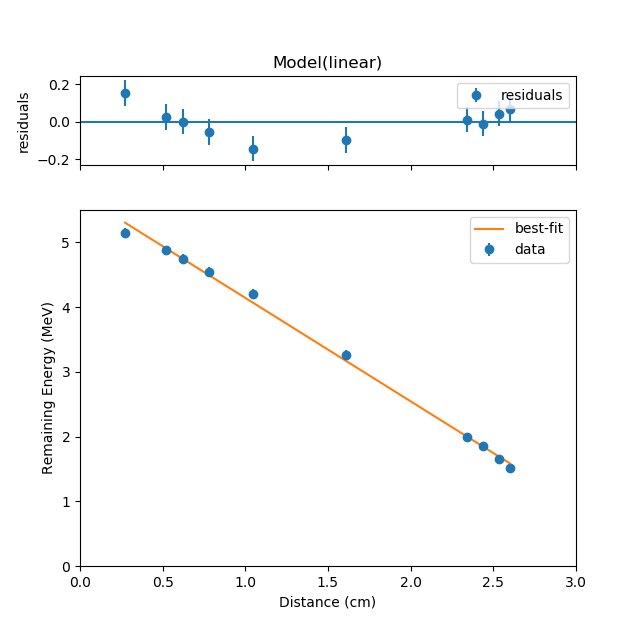
\includegraphics[scale=0.7]{grafiek_lucht}
\caption{De overgebleven energie van de alfadeeltjes na een bepaalde afstand door lucht met atmosferische druk gereisd te hebben. De helling van de fitlijn bepaalt de stopping power.}
\label{fig:figuur1}
\end{figure}

\newpage

Zie figuur \ref{fig:figuur2} voor de resultaten van de metingen met helium.
Voor de stopping power van helium bij atmosferische druk volgt uit de lineaire fit aan de data:
\begin{equation}
\text{stopping power}_\mathrm{helium} = 215 \text{ keV/cm} \pm 4 \text{ keV/cm}
\label{eq:stopping_power_lucht}
\end{equation}
De gereduceerde $\chi^2$ van de fit is 1,08. Voor de dracht in helium volgt:
\begin{equation}
R_\mathrm{\alpha, helium} = 25,4 \text{ cm} \pm 0,5 \text{ cm}
\label{eq:range_air}
\end{equation}

\begin{figure}  % Forceer je figuur niet naar [h]ere. Dat gebeurt in artikelen ook niet.
\centering
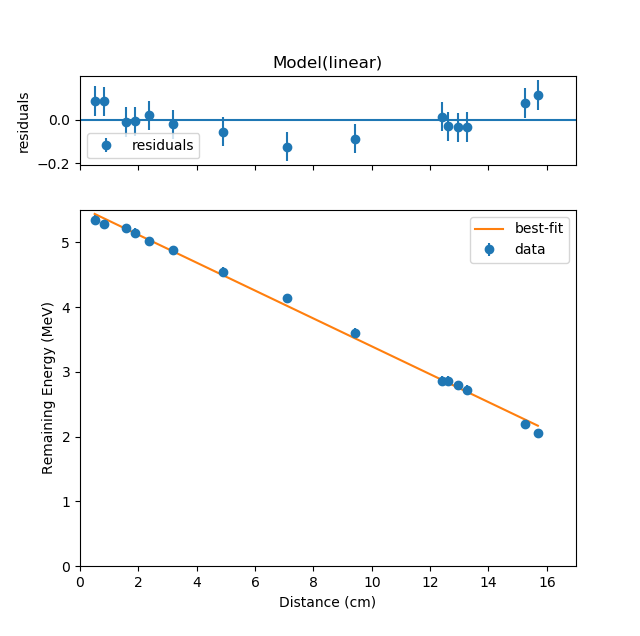
\includegraphics[scale=0.7]{grafiek_helium}
\caption{De overgebleven energie van de alfadeeltjes na een bepaalde afstand door helium met atmosferische druk gereisd te hebben. De helling van de fitlijn bepaalt de stopping power.}
\label{fig:figuur2}
\end{figure}

\newpage

\section*{Conclusie \& Discussie}
De p-waarde voor de fit van lucht is 0,08. Op basis van een significantielevel van 0,05 hoeft de fit dus niet verworpen te worden. Ook de fit van helium hoeft op basis van hetzelfde significantielevel niet verworpen te worden, want de p-waarde is hier 0,37.

De berekende stopping power van zowel lucht als helium zit niet binnen 20\% van de theoretische waarde. Bij de berekende dracht in beide stoffen is dit wel het geval.

Het feit dat de berekende stopping powers niet overeen komen met de theoretische waardes kan liggen aan een systematische fout in de opstelling. Om deze fout te verkleinen kan de ratio lucht:helium bepaald worden voor zowel de theoretische als de berekende waardes. Bij de theoretische waardes is deze ratio 6,97, en bij de berekende waardes 7,42. Dit ligt redelijk bij elkaar in de buurt, dus het verschil in berekende en theoretische waarde zou voor een deel door de systematische fout in de opstelling veroorzaakt kunnen worden. Aantekening hierbij is wel dat de theoretische waardes uit twee verschillende artikelen gehaald zijn, en hier dus ook een andere systematische fout in de opstelling gezeten kan hebben. Meer onderzoek is nodig om te achterhalen wat de systematische fout in de opstelling is.

De detector is geijkt met maar 1 waarde, omdat alleen de meest voorkomende alfadeeltjes duidelijk uit het histogram gehaald konden worden. Om het aantal pulshoogtes per MeV nauwkeuriger te kunnen bepalen, zou de detector met meerdere bronnen geijkt moeten worden. Zo kan er aan meer energieën gefit worden. Ook is het dan mogelijk een fout op het aantal pulshoogtes per MeV te bepalen.

%\section{Figuren en tabellen}
%Een voorbeeld van een figuur is op de volgende pagina gegeven, %zie figuur \ref{fig:figuur1}. Figuren staan nóóit in de lopende tekst. Pak een willekeurig artikel en je zult zien dat figuren óf bovenaan een pagina staan, óf onderaan een pagina, óf op een eigen pagina. Nooit in het midden. Probeer dus ook niet met \verb|[h]| o.i.d. de plaatsing van figuren te forceren. Over het algemeen maak je het alleen maar erger.

%\begin{figure}  % Forceer je figuur niet naar [h]ere. Dat gebeurt in artikelen ook niet.
%\centering
%\includegraphics[scale=0.5]{figuur1}
%\caption{Een figuur heeft een onderschrift. Een plaatje trekt al snel je aandacht weg van de hoofdtekst. Zodra je het plaatje snel bekeken hebt, is de natuurlijke neiging om `verder te lezen' en beweegt je aandacht naar onder het plaatje. Als dáár dan een stukje tekst met uitleg staat, wordt het sneller gelezen dan wanneer dat bóven de figuur staat. Blijkt uit onderzoek.}
%\label{fig:figuur1}
%\end{figure}

%Een voorbeeld van een tabel is hieronder gegeven, zie tabel \ref{tab:tabel1}.

%\begin{table}
%\caption{Een tabel heeft een bovenschrift. Een plaatje of tabel (met veel witruimte eromheen) trekt al snel je aandacht weg van de hoofdtekst. Toch worden je ogen al snel richting de kop getrokken (wat staat er boven de kolommen?) en als dáár dan een stukje tekst met uitleg staat, lees je dat sneller dan wanneer het ónder de tabel staat. Blijkt uit onderzoek.}
%\centering
%\begin{tabular}{SS} % uitlijnen als getal, dus met de komma's b.v. recht onder elkaar.
%\toprule
%{Slingerlengte [\si{\centi\meter}]} & {Slingertijd [\si{\second}]} \\  % Kop moet tussen {} om uitlijning als getal te voorkomen
%\midrule
%5 & 4.5 \\
%10 & 6.3 \\
%15 & 7.8 \\
%20 & 9.0 \\
%25 & 10.0 \\
%\bottomrule
%\end{tabular}
%\label{tab:tabel1}
%\end{table}

%\section{Een sectie}

%Formules in \LaTeX\ gaan vanzelf al snel goed. Zo krijgt iedere vergelijking automatisch een nummer, dat keurig rechts wordt uitgelijnd. Menig student krijgt dat in Word o.i.d. niet goed voor elkaar. Denk er wel aan formules op te nemen in de lopende tekst.
%\begin{equation}
%  F = ma
%  \label{eq:eerste-wet-newton}
%\end{equation}
%De eerste wet van Newton. Vergelijking \ref{eq:eerste-wet-newton} is níet opgenomen in de lopende tekst, en dat leest dus niet zo lekker door. Je moet jezelf afvragen: kan ik dit verhaal voorlezen? Als je het verhaal goed kunt voorlezen \emph{inclusief} de vergelijking, zonder haperingen, dan staat het goed.

%Zo is bijvoorbeeld de trillingstijd van een slinger gegeven door
%\begin{equation}
%  T = 2\pi\sqrt{\frac{l}{g}},
%  \label{eq:trillingstijd-slinger}
%\end{equation}
%met de trillingstijd $T$, de lengte van de slinger $l$ en de valversnelling $g$. Let ook op de komma aan het eind van vergelijking~\ref{eq:trillingstijd-slinger}. Dit stukje tekst kun je vloeiend voorlezen, zonder haperingen. Geef je vergelijkingen ook \emph{namen} om aan te refereren, en geen \emph{nummers}.

%Lorem ipsum dolor sit amet, consectetur adipiscing elit. Ut tempor ullamcorper sapien, quis lacinia nibh pellentesque vel. Sed ultrices nunc vitae magna pulvinar ac posuere velit bibendum. Nunc placerat ornare libero nec viverra. Nulla ullamcorper diam orci, sit amet scelerisque nisl. Nam sapien felis, auctor vestibulum dignissim nec, egestas eget dolor. Suspendisse iaculis, diam pulvinar luctus iaculis, ipsum nisl consectetur nisi, a lacinia eros lacus vitae dui. In fermentum ante quis ante porttitor congue. Mauris sollicitudin rhoncus dictum. Donec pretium molestie tempus. Integer suscipit egestas erat sit amet volutpat. Nullam et magna risus. Nam vel nisi libero. Duis ultricies ipsum eu lorem congue vestibulum. Aenean ut felis velit, ac lacinia erat. In a dolor dignissim elit faucibus facilisis. Vivamus iaculis ornare lacus, viverra convallis sapien pulvinar vitae.

%\section{Referentie voorbeelden}

%\citet{Kachru2003} hebben aangetoond dat de Sitter vacua voorkomen in snaartheorie. Dit werd echter in een latere publicatie tegengesproken \citep{Bena2010}.

%Refereren met LaTeX kan op twee manieren, zie ook Hoofdstuk 5 van de handleiding AVT. Hier voegen we referenties handmatig toe door gebruik te maken van thebibliography, zie de regels hieronder beginnend bij \begin{thebibliography}{}. Elke nieuwe referentie wordt toegevoegd met \bibitem.

%In een \bibitem geeft de tekst tussen de [...] aan hoe de referentie verschijnt in de tekst. Tussen de {...} staat het label waarmee in de tekst naar de referentie kan worden verwezen. Refereren in de tekst wordt gedaan zoals hierboven (met \citet{<label>} en \citep{<label>}).

%\begin{thebibliography}{}
%\bibitem[Kachru \emph{et al.}(2003)]{Kachru2003} Kachru, S., Kallosh, R. \& Linde, A., De Sitter vacua in string theory, 2003, Phys.Rev., D68, 046005
%\bibitem[Bena \emph{et al.}(2010)]{Bena2010} Bena, I., Grana, M., \& Halmagyi, N., On the Existence of Meta-stable Vacua in Klebanov-Strassler,  2010, JHEP, 1009, 087
%\end{thebibliography}

\end{document}
